\chapter[Extending the JastAdd Extensible Java Compiler to Java 7]{\texorpdfstring{%
Extending the JastAdd Extensible Java Compiler\\to Java 7}{%
Extending the JastAdd Extensible Java Compiler to Java 7}}
\label{ch:java7}
\paperRemark{\paperIref}

{

\section*{Abstract}

JastAddJ is an extensible Java compiler, implemented using reference attribute
grammars. It has been shown previously how the language constructs of Java~5,
like generics, could be modularly added to the original JastAddJ compiler that
supported Java~1.4.

In this paper we discuss our experiences from extending JastAddJ to support
Java~7. In particular, we discuss how the Try-With-Resources statement and the
Diamond operator could be implemented, and how efficient the resulting Java~7
compiler is regarding code size, compilation time, and memory usage.

\section{Introduction}

The Java language has gone through several updates, including versions 1.4, 5, 6, 7,
and currently 8, each adding new constructs or standard class libraries to the
language. Each new language version requires compiler support.  While a
state-of-the art compiler, like OpenJDK, implements such updates by modifying
the source code of the previous version of the compiler, it has been shown how
\emph{reference attribute grammars} \cite{DBLP:journals/informaticaSI/Hedin00} (RAGs) can be used to
build extensible compilers, where new language constructs can be added
modularly, without changing the previous source modules. In particular,
\emph{JastAddJ} is an extensible compiler for Java, implemented using
\emph{JastAdd}, a metacompilation system that supports RAGs \cite{jastadd}.
JastAddJ originally supported Java~1.4, but was extended modularly to support
all Java~5 features -- enums, the enhanced for-statement, autoboxing, varargs,
static imports, generics with wildcards, and annotations \cite{jastaddj}.

The ability to modularly add language constructs has many advantages. For
example, several versions of a language can be supported simultaneously without
duplicate code, and researchers can reuse a compiler with relative ease, to construct new
language extensions or tools. There are many examples of research languages
that have been implemented on top of JastAddJ, e.g., \emph{abc} (the
AspectBench Compiler) \cite{abc08}, \emph{JCop} (a context-oriented programming
extension to Java) \cite{jcop10}, and \emph{Fuji} (an extensible compiler for
feature-oriented programming in Java) \cite{fuji12}.

In this paper, we describe how we have modularly extended JastAddJ to support
Java~7. We focus on the implementation of the two constructs we found the most
challenging to implement, \emph{Try With Resources} (TWR), and the
\emph{Diamond} operator. We were particularly aided by the use of
\emph{higher-order attributes} \cite{vogt1989higher}, i.e., computed abstract
syntax tree values.

%We describe these extensions in terms of two recurring patterns that we have found generally useful, namely \emph{Delegated Code Generation} that allows code generation for a new construct to be delegated to a similar existing construct, and \emph{Reified Type} that allows implicit types to be reified on demand in the compiler. Both patterns make use of \emph{higher-order attributes} \cite{vogt1989higher}, i.e., computed abstract syntax tree values.

We evaluate the resulting compiler by investigating code size, compilation
time, and memory usage, both as compared to the Java~6 version of JastAddJ and
to the Java~7 version of OpenJDK.

The remainder of this paper is organized as follows. Section \ref{JastAddJ}
gives background information on the JastAddJ compiler. Sections \ref{TWR} and
\ref{Diamond} describe how the TWR and Diamond constructs were implemented. Section \ref{sec:evaluation} evaluates the
implementation and section \ref{sec:related-work} discusses related work. The paper
is concluded in section \ref{java7:sec:conclusions}.

\section{The JastAddJ Compiler}
\label{JastAddJ}

The \emph{JastAddJ} compiler, \cite{jastaddj} is a Java compiler developed to demonstrate
extensible compiler development using reference attribute grammars (RAGs) \cite{DBLP:journals/informaticaSI/Hedin00}.

\subsection{Overall architecture}

The compiler was initially developed for Java~1.4, and later extended to Java~5, 6, and 7. An extension to Java~8 is ongoing work. The development has recently been moved to bitbucket, at \texttt{https://bitbucket.org/jastadd/jastaddj}, and there is one source directory for each Java version: \texttt{java4}, \texttt{java5}, \texttt{java6}, and \texttt{java7}. Each such directory contains subdirectories containing the specifications for \texttt{scanner}, \texttt{parser}, \texttt{grammar} (for the abstract syntax tree), \texttt{frontend} (static-semantic analysis), and \texttt{backend} (byte code generation). The scanners are implemented in JFlex \cite{jflex}, the parsers in Beaver \cite{beaver}, and the grammars, frontends, and backends are implemented in the JastAdd metacompilation tool, using RAGs \cite{jastadd}. Figure \ref{JastAddJLOCs} shows the number of source lines of code (excluding whitespace and comments) in these directories.

\begin{figure}
\center
\small
\begin{tabular}{ | l | r | r | r | r || r | r |}
\hline
  & \emph{java4} & \emph{java5} & \emph{java6} & \emph{java7}& \textbf{total} & \textbf{\%}\\
  \hline
  scanner & 308 & 17 &  & 109 & \textbf{437} & 2\\
  \hline
  parser & 763 & 537 &  & 102 &\textbf{1402} & 5\\
  \hline
  grammar & 167 & 57 &  & 21 &\textbf{245} & 1\\
  \hline
  frontend & 9409 & 6178 & 27 & 1725 &\textbf{17573} & 65\\
  \hline
  backend & 5505 & 1321 &  & 443 &\textbf{7250} & 27\\
  \hline
  \hline
  \textbf{total} & \textbf{16150} & \textbf{8110} & \textbf{27}& \textbf{2400}&\textbf{26687} & 100\\
  \hline
\end{tabular}
\caption{Lines of code for JastAddJ modules. Excludes whitespace and comments.}
\label{JastAddJLOCs}
\end{figure}

% breäknat mha. sloccount.sh i jastaddj

We can note that the major part of the total code is in the frontend  (65\%),
and the next largest part is the backend (27\%). The Java~6 addition is very
small: most of the new features in Java~6 concerned libraries, and the only
change to the language was a change in the semantics of the \texttt{Override}
annotation.

To generate the Java~7 compiler,  the scanner modules are combined and then
processed by JFlex,  the parser modules are combined and then processed by
Beaver, and the grammar, frontend, and backend modules are passed to JastAdd.
The resulting generated Java source files are compiled together with around
1800 lines of driver code, written in Java.  The driver code includes a Unicode
scanner, Beaver runtime classes, and entry points for the Java compiler, static
semantic checker, pretty printer and corresponding Ant tasks.  The driver code
is reused for all versions of the compiler.

\subsection{Reference attribute grammars}

It is the use of reference attribute grammars (RAGs) that makes it possible to
modularize the different Java support levels in Jast\-AddJ. A RAG specifies
abstract syntax trees (ASTs), decorated with attributes that are defined using
equations.  The specification is \emph{declarative} in the sense that in any correctly
attributed AST all attributes will have values such that all equations are
satisfied. The specification order of attributes and equations is thus
irrelevant. The specification is also \emph{executable}: an evaluator that
computes the correct attribution can be automatically generated from the RAG.
RAGs differ from Knuth's original attribute grammars \cite{Knuth68} in that
attributes may have \emph{reference} values, i.e., they may refer to other
nodes in the AST, and they may be \emph{parameterized}, i.e., they may take
arguments. Reference attributes are useful for representing graph structures on
top of the AST, e.g., for linking a use of a variable to its declaration node.
In JastAdd, there are also additional attribution mechanisms, in particular,
higher-order attributes \cite{vogt1989higher}, also known as \emph{non-terminal
attributes} (NTAs). An NTA is an attribute whose value is an AST subtree, and
which can itself have attributes. NTAs are useful for computing AST structures
during compilation, for example for macro expansions or similar problems. In
JastAdd, NTAs can be parameterized, just like ordinary attributes.

Like in Knuth's attribute grammars, an attribute can be either synthesized or inherited. For \emph{synthesized} attributes, the defining equation must be located in the same node as the attribute. In contrast, if an attribute is declared as \emph{inherited}, the responsibility to define the attribute is delegated to the context, i.e., to the parent of the node. In JastAdd, this responsibility is automatically delegated transitively through the parent chain until a node is found with an equation defining the attribute.

The attributed AST is the main data structure used in the Jast\-AddJ compiler.
For example, instead of using traditional symbol tables, declarations in a
program are simply represented by the corresponding AST nodes through reference
attributes that can locate the declaration from a use site. If the AST
constructed by the parser is not sufficient for representing some information
conveniently, additional structure can be added through NTAs. The advantage of
this approach is that all information can easily be extended or overridden by
other modules, through the RAG mechanisms.

%\subsection{RAG frameworks}

To add a new language construct, one or more new RAG modules are added with new
node types, attributes and equations. Through aspect-oriented inter-type
declarations \cite{1997aspect}, attributes and equations in the new modules can
apply to the new types as well as to types in the existing modules.  A RAG
specification is in many ways similar to an object-oriented framework: the AST
node types are actually an object-oriented (Java) class hierarchy. The
attributes can be called as methods, and equations defining attribute values
can be overridden in subclasses, similar to Java methods.

We have implemented the Java~7 features as a JastAddJ extension. Figure
\ref{fig:scope} shows which parts of JastAddJ were extended by each new Java~7
feature, and how many lines of code were needed.

The Improved Numeric Literals feature required relatively many lines of code
due to a refactoring made to the parsing of numeric literals that replaced old
non-attribute grammar code.

\begin{figure}
\adjustbox{center}{
\small{
\begin{tabular}{|l|c|c|c|c|c|c|}
    \hline
    \emph{Feature} & \emph{scanner} & \emph{parser} &
    \emph{grammar} & \emph{frontend} &
    \emph{backend} & \emph{Total} \\
    \hline
    Try-With-Resources & & 54 & 4 & 181 & 150 & 389 \\
% TWR         54 java7/parser/TryWithResources.parser
% TWR         1 java7/grammar/BasicTWR.ast
% TWR         3 java7/grammar/TryWithResources.ast
% TWR         24 java7/frontend/Variable.jadd
% TWR         157 java7/frontend/TryWithResources.jrag
% TWR         150 java7/backend/TryWithResources.jrag

    \hline
    Strings in Switch & & & & 41 & 229 & 270 \\
% SIS         41 java7/frontend/StringsInSwitch.jrag
% SIS         229 java7/backend/StringsInSwitch.jrag

    \hline
    Diamond & & 6 & 2 & 327 & & 335 \\
% DIAMOND     6 java7/parser/Diamond.parser
% DIAMOND     2 java7/grammar/Diamond.ast
% DIAMOND     327 java7/frontend/Diamond.jrag

    \hline
    Improved Numeric Literals & 111 & 20 & 11 & 932 & & 1074 \\
% NUMERICLIT  49 java7/scanner/Macros.flex
% NUMERICLIT  62 java7/scanner/Literals.flex
% NUMERICLIT  20 java7/parser/Literals.parser
% NUMERICLIT  11 java7/grammar/Literals.ast
% NUMERICLIT  327 java7/frontend/ConstantExpression.jrag
% NUMERICLIT  605 java7/frontend/Literals.jrag

    \hline
    Multi-catch & & 22 & 4 & 190 & 60 & 276 \\
% MULTICAT    22 java7/parser/MultiCatch.parser
% MULTICAT    4 java7/grammar/MultiCatch.ast
% MULTICAT    190 java7/frontend/MultiCatch.jrag
% MULTICAT    60 java7/backend/MultiCatch.jrag

    \hline
    More Precise Rethrow & & & & 174 & 4 & 178 \\
% RETHROW     174 java7/frontend/PreciseRethrow.jrag
% RETHROW     4 java7/backend/PreciseRethrow.jrag

    \hline
    Safe Varargs & & & & 86 & & 86 \\
% VARARGS     17 java7/frontend/Warnings.jadd
% VARARGS     69 java7/frontend/SafeVarargs.jrag

    \hline
    Miscellaneous & & & & 69 & & 69 \\
% MISC        23 java7/frontend/JastAddExtensions.jadd
% MISC        16 java7/frontend/SuppressWarnings.jrag
% MISC        25 java7/frontend/UncheckedConversion.jrag
% MISC        5 java7/frontend/PrettyPrint.jrag

    \hline
    \textbf{Total} & \textbf{111}& \textbf{102}& \textbf{21}& \textbf{2000}& \textbf{443} & \textbf{2677}\\
    \hline
\end{tabular}
}
}%adjustbox
\caption{Lines of code needed for the different Java~7 features (excluding whitespace and comments).}
\label{fig:scope}
\end{figure}

%The Java~1.4, 5, and 6 modules together constitute a RAG framework that is
%extended by the Java~7 modules. Figure XXX shows key parts of this framework
%and the Java~7 extension.

%\textbf{TODO}: Draw some key classes with synthesized and inherited attributes,
%and describe this. Draw the things that are needed in order to explain most of
%the TWR and Diamond extensions.



\section{Try With Resources}
\label{TWR}

The \emph{try-with-resources} (TWR) statement was added to the Java language to
reduce the code clutter from closing a resource, particularly resources that
can throw exceptions when closed.

\vbox{
Before Java~7 the following code would be required to ensure that a resource
was closed properly:

\begin{lstlisting}[deletekeywords={throw}]
Resource resource = null;
try {
    resource = new Resource(); // may throw
    // use resource here
} finally {
    if (resource != null) {
        try {
            resource.close(); // may throw
        } catch (IOException e) {
        }
    }
}
\end{lstlisting}
}

The TWR statement is similar to a regular \verb'try' statement --
it can have catch clauses and a finally clause -- but with an extra resource
declaration part where one or more resources are declared and initialized.
Using TWR we can rewrite the above example to the following:

\begin{lstlisting}
try (Resource resource = new Resource()) {
    // use resource here
}
\end{lstlisting}

When control passes out of a TWR statement all resources opened in the resource
declaration part will be auto-closed. This occurs even if the TWR completes
abruptly (e.g., due to an exception).

\subsection{TWR static semantics}

%To implement the static semantics for TWR, we introduced a new node type  \verb'TryWithResources' as a subclass of the existing \verb'TryStmt'.
The JastAddJ framework for Java~1.4 contains a class modeling the regular \verb'try' statement (\verb'TryStmt'), containing a main code block, a list of catch clauses, and an optional \verb'finally' clause.
Figure \ref{TWRextension} outlines how the framework was extended in the Java~7 frontend to support static semantics for TWR. A new node class \verb'TryWithResources' was introduced that extends \verb'TryStmt' with a list of resource declarations, modeled as a new subclass of the existing class \verb'VariableDeclaration'. Most of the behavior in  \verb'TryStmt' is reused, but a few declarations are added in the extension, in order to adapt the behavior for TWR. For example, name analysis and analysis of reachability, exception handling, and definite assignedness is adapted.

%These adaptations concern, for example, name analysis, reachability analysis, exception handling analysis, definite assignedness analysis, and error checking, as explained in the following.

The name analysis is adapted to make the resource declarations visible in the
main block of the TWR. This is accomplished through the addition of an equation
in \verb'TryWithResources' that redefines the inherited attribute
\verb'lookupVariable' of the block. This attribute is used to look up
declarations for variable uses inside the block. In a similar way, the
reachability analysis (of TWR catch clauses) and exception handling checking
(of resource initialization and closing exceptions) are handled by adding new
equations that define or redefine inherited attributes of children of the TWR.

The definite assignedness analysis in JastAddJ uses a synthesized attribute \texttt{s.isDAbefore(v)} and an inherited attribute \texttt{s.isDAafter(v)} to define if a variable \texttt{v} is definitely assigned before/after a statement \texttt{s}. The TWR extension includes equations that (re-)define \texttt{isDAafter} for the TWR statement, and \texttt{isDAbefore} for the children, in order to take the resource declarations into account.

%reusing most of  the attributes and equations. To make the resource declarations visible in name- and type analysis, we implemented an equation for the inherited attribute \verb'lookupVariable'.

%The semantics of TWR are also very similar to the \verb'try' statement, so we
%extended the \verb'TryStmt' node type in JastAddJ to create the new
%\verb'TryWithResources' node type. Most of the semantic analysis attributes did
%not have to be altered, but in order to make the resource declarations visible
%in name- and type analysis we implemented an equation for the inherited
%attribute \verb'lookupVariable'.
%We also had to implement reachability analysis
%(of TWR catch clauses), exception handling checking (of resource initialization
%and closing exceptions), and definite assignedness checking (of resources) by
%specializing related synthesized attributes and methods for the TWR statement.

There are new kinds of possible compile-time errors for TWR statements. An
example is declaring a resource of a type that does not implement
\verb'AutoCloseable' (a new interface that declares the \verb'close' method
used to close a resource). JastAddJ collects compile-time error messages
through calling the method \texttt{typeCheck} on all nodes. This method is
implemented for \texttt{ResourceDeclaration} in order to check for these
errors.

\begin{figure}
	\centering
	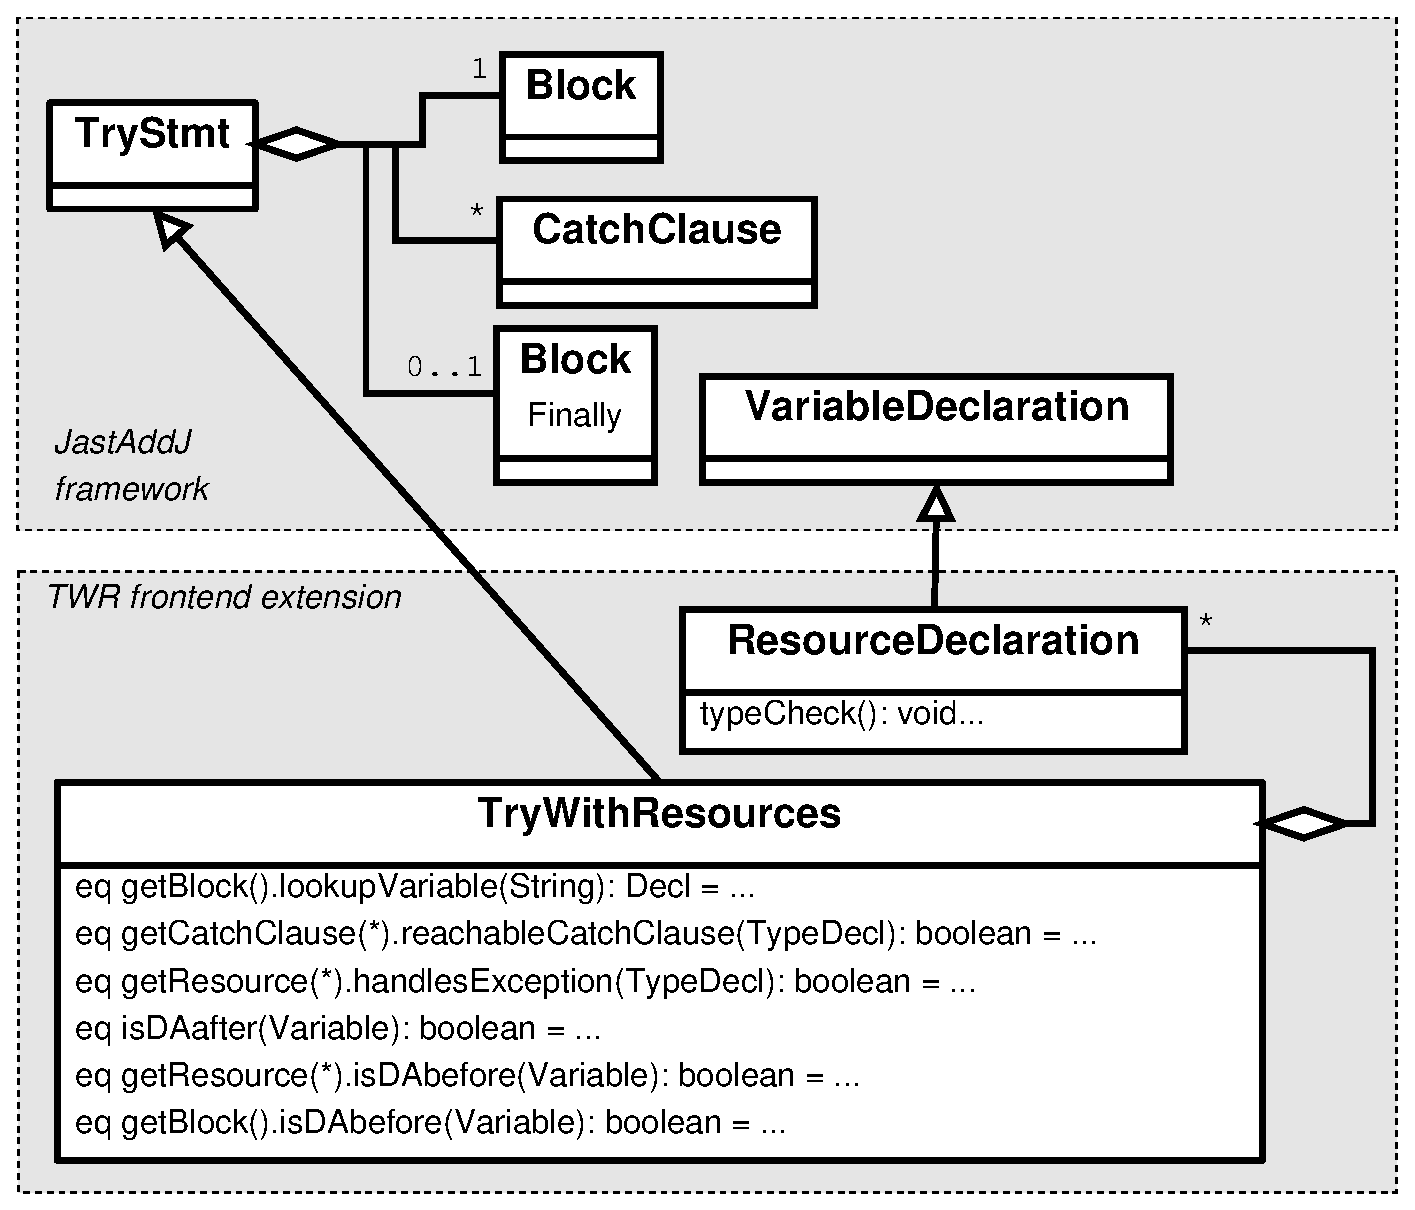
\includegraphics[width=\columnwidth]{figures/TWRextension.eps}
	\caption{\texttt{TryWithResources} and \texttt{ResourceDeclaration} are two new node types added to support TWR. The static semantics of TWR is adapted through equations and other declarations.}
	\label{TWRextension}
\end{figure}

\subsection{TWR code generation}

While the \verb'TryWithResources' node type conveniently describes the static semantics of the
TWR statement, implementing code generation was trickier.
The TWR statement does many things implicitly that need explicit code
generation support.  The Java bytecode does not have built-in support for
auto-closing resources, so all the steps needed for managing resources
correctly need to be generated into bytecode.

The approach we used in JastAddJ builds on the fact that any TWR statement can be transformed into a regular \texttt{try} statement with a series of basic TWR statements nested inside it, as described in the Java Language Specification \cite[p. 408]{jls7}. A \emph{basic TWR} statement has no catch clauses or finally clause--it has only resource declarations and a block. By transforming a TWR statement this way, the bytecode generation for the \texttt{try} statement can be reused, and the generation of the autoclosing support can be implemented in a simple way for the basic TWR nodes.

We implemented this approach by introducing the transformed version of the TWR statement as a \emph{non-terminal attribute} (NTA), i.e., an attribute whose value is a new AST subtree. The original TWR is used for static-semantic analysis, allowing any compile-time errors to be more closely related to the original source code. The code generation for a TWR is delegated to the transformed version of the statement, i.e., to the NTA. Figure~\ref{TWRbackend} outlines the extensions done in the Java~7 backend. Note that the NTA and the code generation method are added to the \texttt{TryWithResources} node type using \emph{inter-type declarations}. Inter-type declarations allow features of classes to be added in separate modules \cite{1997aspect}.

\begin{figure}
	\centering
	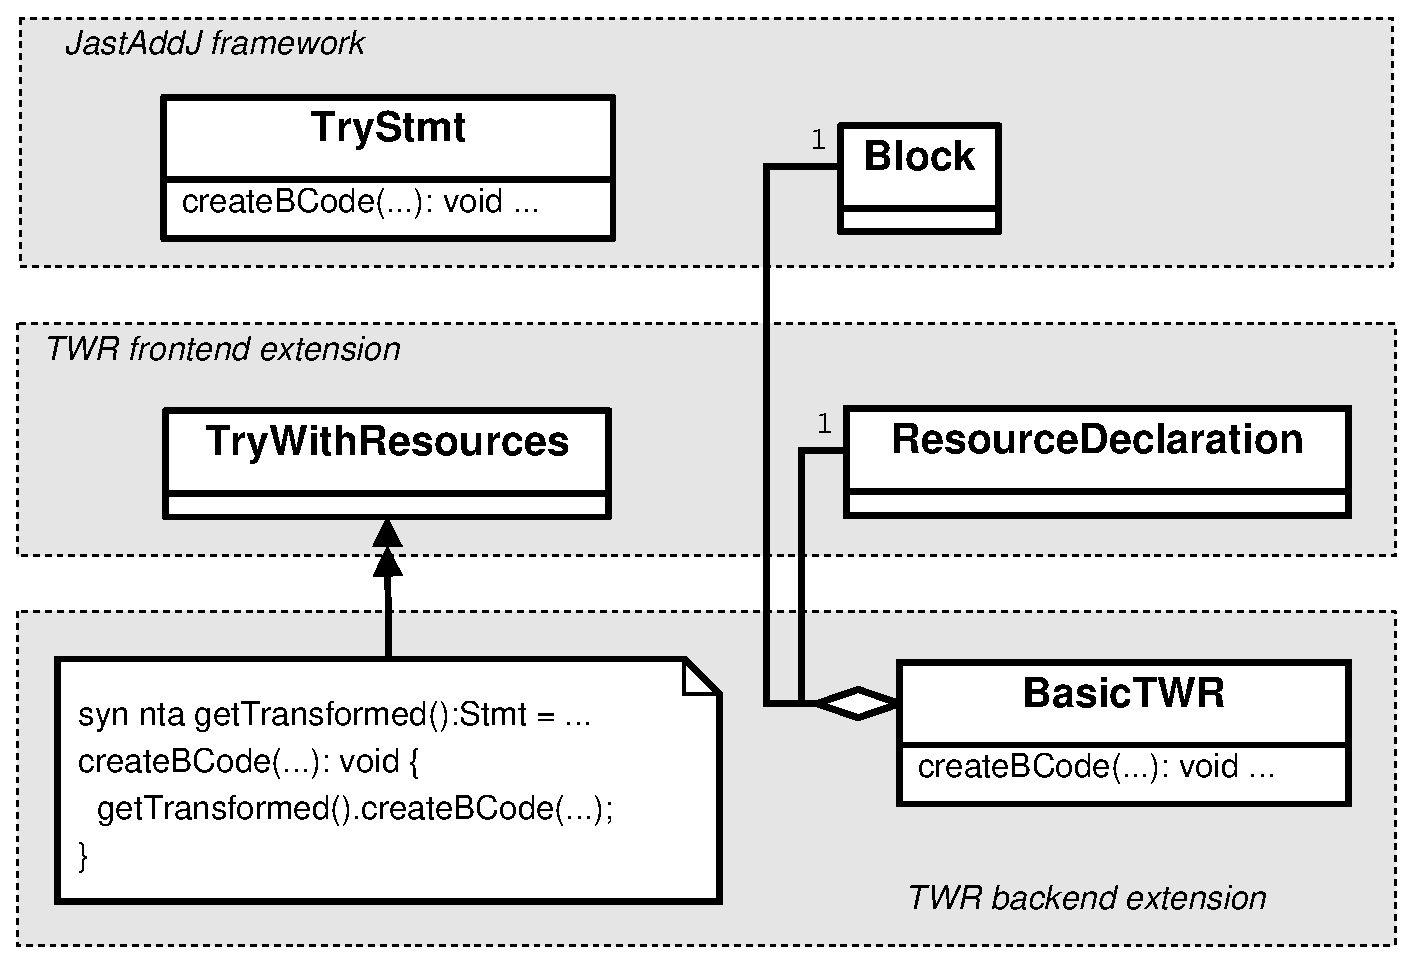
\includegraphics[width=\columnwidth]{figures/TWRextensionBackend.eps}
	\caption{To implement code generation for TWR, a \texttt{BasicTWR} node type is introduced, whose code generation handles autoclosure. The code generation method for the TWR statement delegates to the NTA \texttt{getTransformed}, which will be either a \texttt{TryStmt} or a \texttt{BasicTWR} statement. The double-arrowed relation indicates features added to an existing class using inter-type declarations.}
	\label{TWRbackend}
\end{figure}

The transformed version of a TWR may contain a new (simpler) TWR which in turn has an NTA containing its transformed version, so the transformation is carried out in several steps. Furthermore, we defined the \texttt{BasicTWR} to include only a single resource declaration, so if the original TWR contains several resource declarations, this will result in a transformed AST with several nested \texttt{BasicTWR} nodes. Figure~\ref{TWRexpansion} shows an example. A TWR (1) with catch clauses and/or a finally block is transformed to a regular \texttt{try} statement (2), including a new simpler TWR statement (3) with only resource declarations and a block. This simpler TWR statement is transformed into a \texttt{BasicTWR} (4) with one resource declaration, and any remaining resource declarations are included in a yet simpler TWR statement (5). This expansion terminates when the last resource declaration is handled by a \texttt{BasicTWR} (6).

%any TWR statement
%can be transformed into a set of nested \verb'try' statements \cite{jsr334}.  Using a
%transformed version of a TWR statement we can reuse the code generation for the
%\verb'try' statement to generate TWR bytecode.

%The transformed version of a TWR statement is introduced in the AST as an
%\emph{non-terminal attribute} (NTA), i.e., an attribute whose value is a new AST subtree. This way, both the original TWR statement, and its transformed counterpart will be part of the AST. The original TWR is used for static-semantic analysis, allowing any compile-time errors to be related to the original source code. The transformed statement is used for bytecode generation, allowing us to reuse the existing code generation for the \texttt{try} statement.

%non-terminal child of the TWR node. We chose to add it as a nonterminal because
%this allows the error messages referene TWR-specific
%semantics, e.g., type errors can report that a resource must be
%\verb'AutoCloseable', rather than just giving a generic type incompatibility
%message.

\begin{figure}
	\centering
	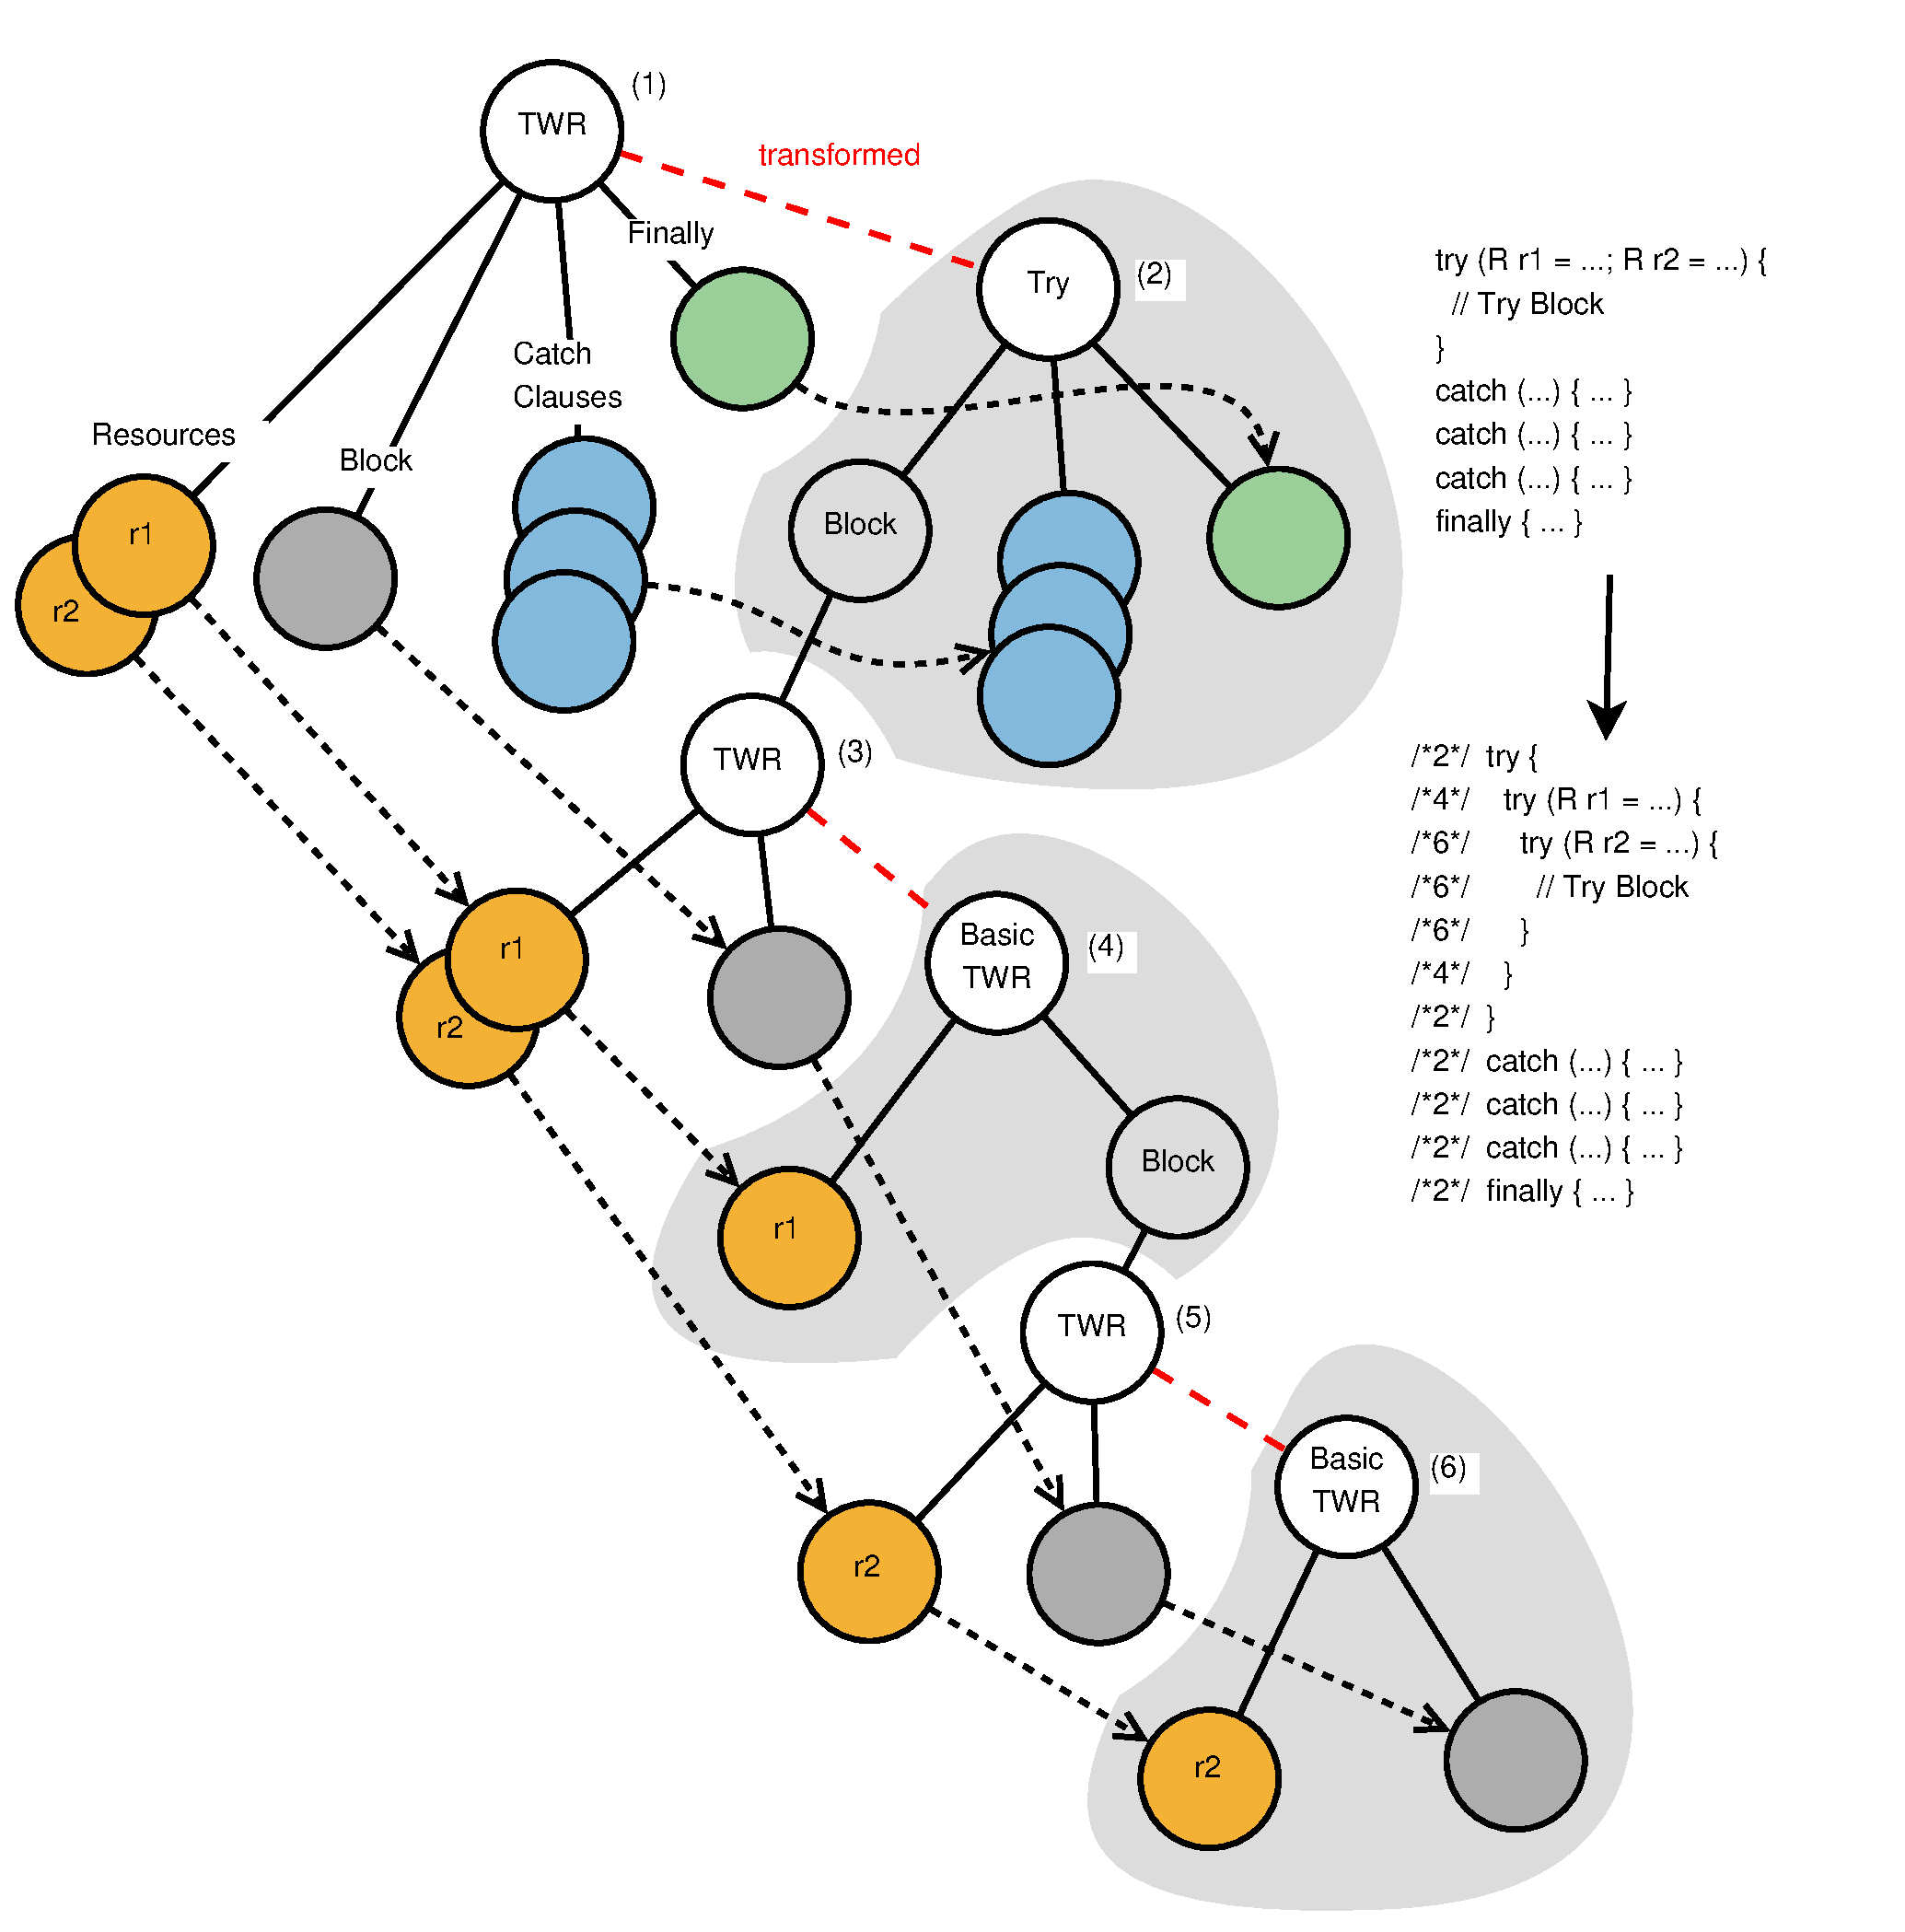
\includegraphics[width=\columnwidth]{figures/TWRtransform.eps}
	\caption{Example of stepwise transformation of a TWR statement using NTAs.
	An NTA \texttt{transformed} contains the new AST for each step.
	Lines without arrowheads indicate child-parent relationships, where the
	red dashed lines indicate NTA children. Dotted black arrows indicate AST
	nodes that are copied into an NTA. Grey shaded areas indicate transformed
	nodes to which code generation is delegated.}
	\label{TWRexpansion}
\end{figure}

%The Java Language Specification defines a special case of the TWR statement
%called \emph{basic} try-with-resources \cite[p. 408]{jls7}.
%A basic TWR statement has no catch clauses or finally clause. The specification
%also gives an equivalent form of the basic TWR statment expressed using
%a try-statement with (in the case of more than one resource declaration) a
%nested basic TWR statement.

%We use the basic TWR in JastAddJ to produce the transformed version of a
%TWR statement. First, the catch clauses and finally clause are moved to an
%enclosing \verb'try' statement. Then, the resulting basic TWR is transformed
%into a series of nested \verb'try' statements. Each transformation step can
%produce a new nested basic TWR, but with one fewer resource declarations than
%the previous basic TWR. This expansion terminates eventually with a simple
%\verb'try' statement.

\section{The Diamond Operator}
\label{Diamond}

In Java~7 the \emph{diamond operator} was added to reduce some of the
redundantly verbose nature of Java generics.

The diamond operator, \verb'<>', allows omission of type arguments for generic
class instance creations in some contexts (assignments, variable/field
initializers, method/constructor arguments). For example, instead of writing

\begin{lstlisting}
List<Integer> myList = new LinkedList<Integer>();
\end{lstlisting}

\noindent
Java~7 allows us to write the following shorter and more readable code:

\begin{lstlisting}
List<Integer> myList = new LinkedList<>();
\end{lstlisting}

%This is a small change, but it makes the code shorter and more readable.

\noindent
The compiler needs to infer omitted type parameters, i.e., \texttt{Integer} in
this case. To accomplish this, we added a new node type, \verb'DiamondAccess',
to represent diamond expressions such as \texttt{LinkedList<>} above.  It is
defined as a subtype of the existing type \verb'Access', allowing it to occur
in a class instance expression, see Figure~\ref{DiamondExtension}.

\begin{figure}
	\centering
	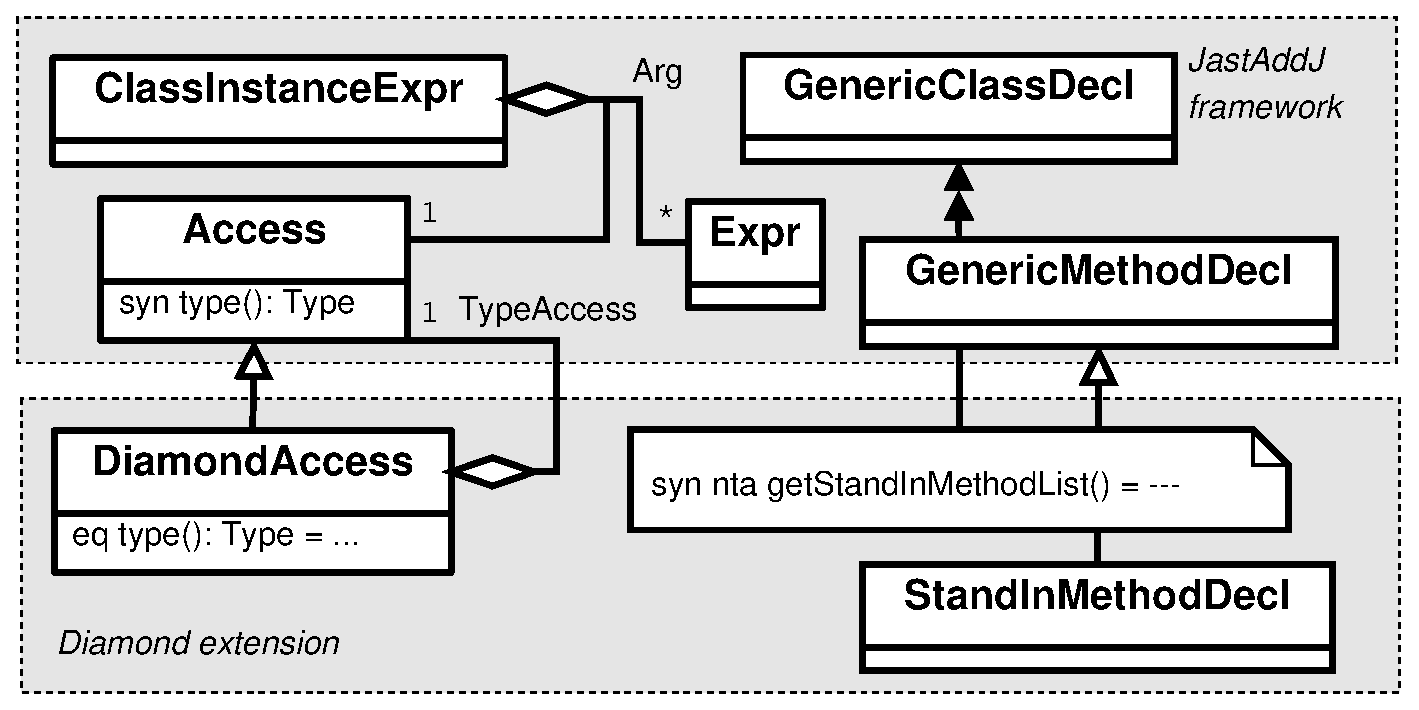
\includegraphics[width=\columnwidth]{figures/DiamondExtension.eps}
	\caption{To support the diamond operator, the JastAddJ frontend is extended with two new node types, \texttt{DiamondAccess} and \texttt{StandInMethodDecl}, and an NTA in the existing type \texttt{GenericClassDecl}.}
	\label{DiamondExtension}
\end{figure}

%When JastAddJ parses a type name followed by an empty
%type argument list it builds a \verb'DiamondAccess' node. The diamond operator
%is only legal if it is part of a class instance expression.

The parent \verb'ClassInstanceExpr' will query its \texttt{Access} child for
its \texttt{type} attribute.  The \texttt{DiamondAccess} node provides an
equation that computes the type attribute by performing type inference: first a
set of candidate constructors is computed, and then the most applicable
constructor and type argument set is found.

It turns out that this problem can be transformed into a similar problem of
inferring method type arguments for generic method invocations, a problem that
was solved already for Java~5. We could implement the diamond inference quite
easily, reusing the existing inference solution by creating a stand-in method
declaration for each candidate constructor.

Figures \ref{DiamondExtension} and \ref{fig:diamond} illustrate the extension.
To represent candidate constructors, a new type, \texttt{StandInMethodDecl} was
added, inheriting from the \texttt{GenericMethodDecl} type used by the existing
type inference algorithm. 

%The type inference for the diamond operator is performed by the
%\verb'DiamondAccess' node. The parent \verb'ClassInstanceExpr' will query it
%for it's type.  When JastAddJ infers type arguments for a diamond operator it
%first computes a set of candidate constructors, then it must find the most
%applicable constructor and type argument set. This problem can be transformed
%into the similar problem of inferring method type arguments for a generic
%method invocation. The inference of generic method type arguments was added to
%the Java language in Java~5 and was previously implemented in JastAddJ, so we
%decided to try to reuse this analysis for the diamond operator.
%
%In order to use the existing inference algorithm we construct a list
%of candidate methods.

A candidate method set is created using all accessible
constructors for the class to be instantiated. Let $C$ be the generic class to
be instantiated, with $T_{1 \ldots n}$ as its type parameters. For each
accessible constructor $K_i$ of $C$ we create a stand-in method $M_i$ with the
same parameter list as $K_i$ and return type $C<T_1, T_2, \cdots, T_n>$. The
stand-in methods $\{M_{1 \ldots m}\}$ are passed to the existing
inference algorithm which computes the most applicable method $M_j$ and
inferred type arguments. This gives us the most applicable constructor ($K_i$)
and the full type argument list for the instance creation. The candidate method
set is represented by a new NTA \verb'getStandInMethodList' added to the type
\verb'GenericClassDecl'.

%The stand-in methods are represented using \verb'MethodDecl' nodes. These are
%computed by the nonterminal attribute  

\begin{figure}
	\centering
	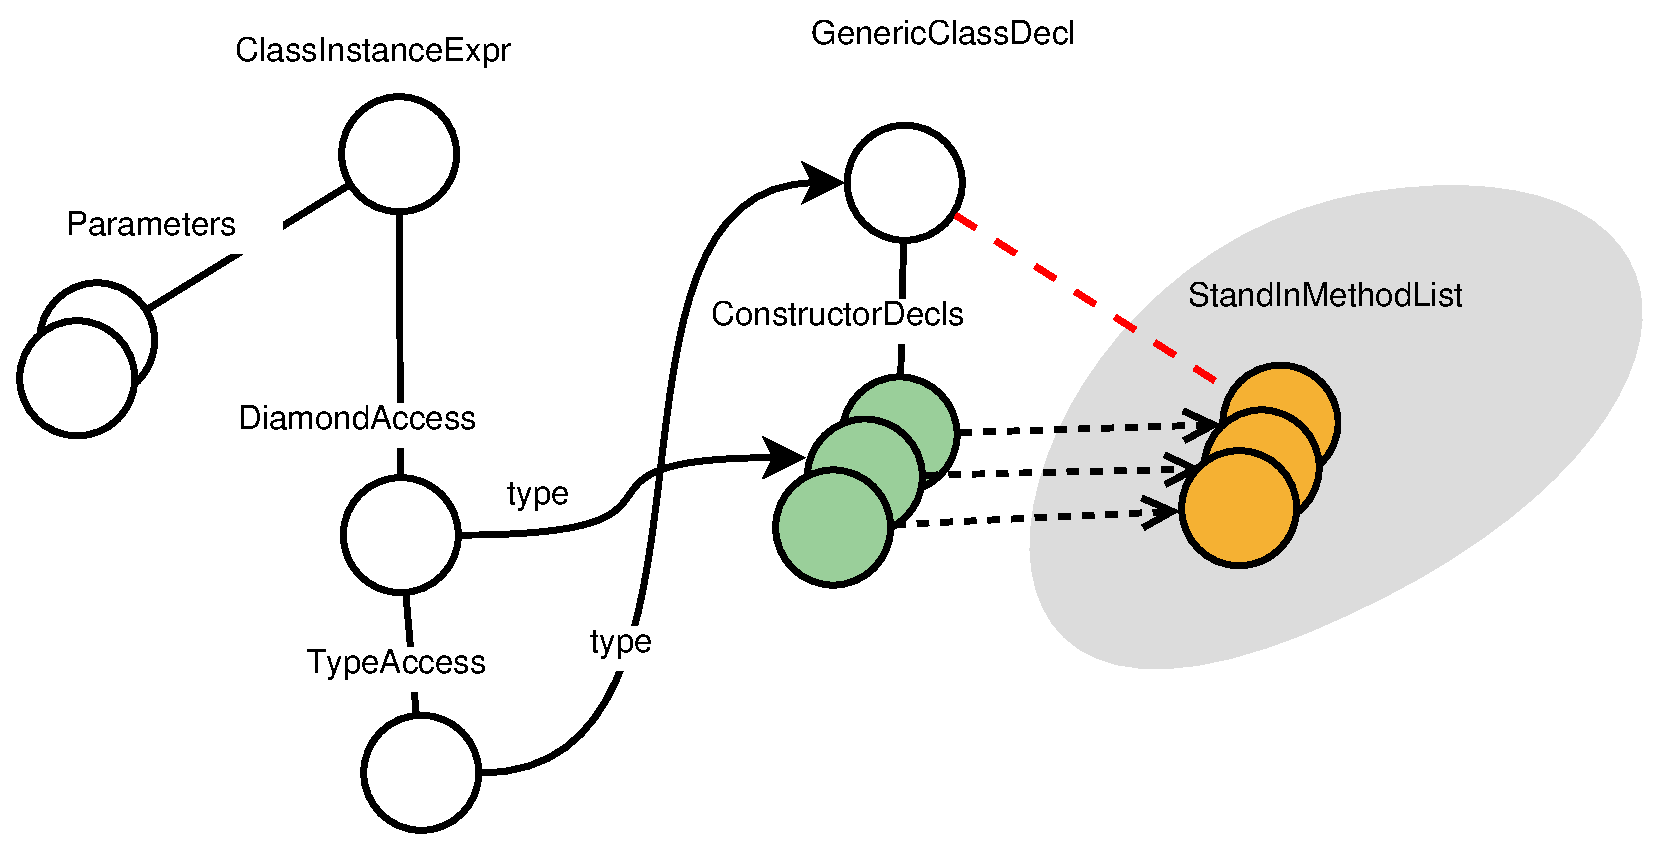
\includegraphics[width=\columnwidth]{figures/Diamond.eps}
	\caption{The Diamond type analysis reuses the Java~5 method type inference by computing stand-in methods using an NTA (the red dashed line). Solid arrows represent the \texttt{type} attributes. Dotted black arrows indicate construction of stand-in method declarations from constructor declarations.}
	\label{fig:diamond}
\end{figure}



\section{Evaluation}
\label{sec:evaluation}

In 2007, JastAddJ was compared to several other Java  compilers, including
Sun's \emph{javac} compiler \cite{jastaddj}. JastAddJ was then found to be less
than three times slower than javac, and with an implementation size of 66\% of
javac (counted in source lines of code). The execution speed of the generated
code was roughly the same for most programs.

Since 2007, both JastAddJ and javac have evolved, so it is interesting to do a
new comparison, and to include the new Java~7 implementations. We have compared
the OpenJDK Java~6 and Java~7 versions of JastAddJ and javac on a number of
different open source benchmark programs. We compare source code size,
compilation speed, memory consumption. We also tested the execution speed of
the generated bytecode, and found that it was almost the same for JastAddJ and
javac, with the JastAddJ-generated code being around 2\% slower on the average. 

The particular versions tested were
builds 7.1.1-49 for JastAddJ (jastaddj-6, jastaddj-7), OpenJDK 6 b24 for
javac-6, and OpenJDK 7 b146 for javac-7.

All tests were carried out on a quad core Intel Core i7-3820 CPU clocked at
3.60GHz with 64 GiB of memory, running Linux Mint with Linux kernel version
3.5.0-17-generic. All measurements were taken using the 64-bit Server editions
of the IcedTea6 1.12.5 (javac-6, jastaddj-6) and IcedTea 2.3.9 (javac-7,
jastaddj-7) runtime environments.  IcedTea is a compatible Java implementation
based directly on the freely available OpenJDK source code.

\subsection{Implementation size}

As an estimate of implementation effort, we have measured the total source code
sizes of JastAddJ and javac, excluding comments and whitespace, using the
tool SLOC-Count \cite{sloccount}. Figure~\ref{ImplementationSize} shows the
results. We see that JastAddJ is just slightly more than half the size of javac: 55\% for Java~6,
and 52\% for Java~7.

%\textbf{TODO:} JastAddJ-6 is now 26 kSLOC, but in the jastaddj article,
%JastAddJ-5 was 21 kSLOC. Why this big difference?? Are the measurements
%correct??

% Jag tror att siffrorna stämmer - jag har mätt om på gamla versioner av JastAddJ
% /Jesper

\begin{figure}[h]
\center
\small
\begin{tabular}{| c | c |}
\hline
\emph{Compiler} & \emph{kSLOC (\% of javac)}\\
\hline
javac OpenJDK 6 b24 & 47.4 (100\%)\\
JastAddJ 7.1.1-49 Java 6& 26.0 (55\%)\\
\hline
javac OpenJDK 7 b146 & 55.1 (100\%)\\
JastAddJ 7.1.1-49 Java 7 & 28.7 (52\%)\\
\hline
\end{tabular}
\caption{The source code size of the compilers, in thousands of source lines of code, and in percentage of javac.}
\label{ImplementationSize}
\end{figure}

\subsection{Compilation speed}

We have measured the mean time to compile a number of different benchmark
programs using Java~6 and 7 versions of javac and JastAddJ. We measured both
the compile time when the compilers are invoked in a fresh Java VM (see section
\ref{fresh-jvm}), as well as the steady-state compile time (section
\ref{steady-state}).

All time measurements were run with 2 GiB heap space, with JIT-compilation
enabled to allow each compiler to run at its optimal performance. The 2 GiB
heap space is well above the minimum required heap space for each benchmark
program (see figure \ref{fig:bm-mem}).

The benchmark programs we have used and their corresponding SLOC counts are
listed in the table in figure \ref{fig:bm-programs}.

\begin{figure}[h]
\centering
\small
\begin{tabular}{|l|l|r|l|}
  \multicolumn{1}{c}{\emph{Name}} &
  \multicolumn{1}{c}{\emph{Version}} &
  \multicolumn{1}{c}{\emph{kSLOC}} &
  \multicolumn{1}{c}{\emph{Description}} \\
  \hline
  %jdepend & 2.9.1 & 2.5 & Java dependency analyzer \\
  junit & 4.5 & 5.2 & Java unit testing framework \\
  jsilver & 1.0.1-SS & 30.1 & HTML template system \\
  %antlr & 2.7.2 & 34.6 & Aspect programming system \\
  clojure & 1.3.0-RC0 & 35.8 & Clojure compiler \\
  lucene & 3.0.1 & 45.3 & Text search engine \\
  javac & jdk7-b146 & 55.1 & OpenJDK 7 javac \\
  jython & 2.2alpha1 & 76.4 & A Python environment in Java \\
  jastaddj & R20111208 & 87.3 & JastAddJ (generated Java code)\\
  \hline
\end{tabular}
\caption{Benchmark programs}
\label{fig:bm-programs}
\end{figure}

\subsubsection{Fresh JVM compilation time}
\label{fresh-jvm}

For each benchmark-compiler pair the benchmark program was compiled 25 times --
each time in a new JVM instance.  The total time to run each invocation of the
compiler was measured (including JVM startup time).  The arithmetic mean of the
measured compile time is presented in figure \ref{fig:bm-time} (labeled without
the \verb'ss-' prefix).  Since JVM startup time was measured as part of the
total compile time we can expect a smaller relative difference in execution
time for the smaller benchmark programs (e.g. junit).

\begin{figure}
	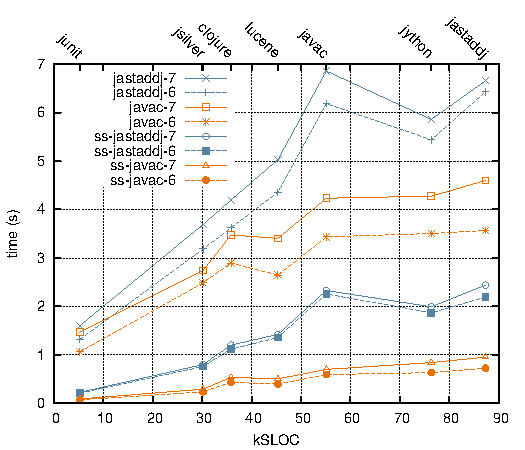
\includegraphics[width=\textwidth]{figures/bm-time}
	\caption{Compilation time. Includes times measured for fresh JVM
	invocations (top four curves) and steady-state execution (bottom four curves). Benchmarks are ordered from left
	to right by increasing SLOC count.}
	\label{fig:bm-time}
\end{figure}

\subsubsection{Steady-state compile time}
\label{steady-state}

We measured steady-state compile time using the method described in
\cite{georges2007statistically}.  A brief summary of the benchmarking
procedure:

\begin{itemize}
	
	\item For each benchmark-compiler pair we run 10 new JVM invocations.

	\item For each JVM invocation the benchmark program is compiled until the
		last 15 measured execution times have a coefficient of variance no
		greater than $0.05$.

	\item The mean of the last 15 compile times for the JVM invocation is
		calculated and stored.

\end{itemize}

The mean steady-state execution time of the 10 JVM invocations for each
benchmark-compiler pair is plotted in figure \ref{fig:bm-time} (labeled with
the \verb'ss-' prefix).

Using a Student's T distribution we calculated the 90\% confidence intervals
for each benchmark and found that they lie within 3\% of the mean execution
time (both for steady-state and fresh JVM).

Much of the time increase from Java~6 to Java~7 compilation is probably due
to the extra parsing time required to parse the larger Java~7 class library.

\subsection{Memory consumption}

We also compared the minimum required JVM heap space to run each
benchmark-compiler combination.  We found the minimum heap space by
doing a binary search from an initial 2048 MiB heap size to the lowest
heap size at which it was still possible to compile the benchmark program.
The minimum measured heap sizes are illustrated in figure \ref{fig:bm-mem}.

\begin{figure}
	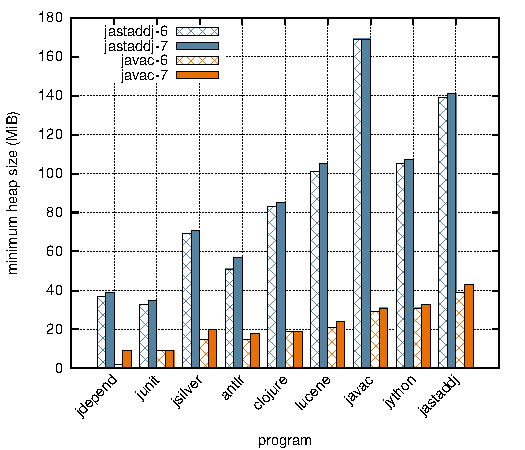
\includegraphics[width=\textwidth]{figures/bm-mem}
	\caption{Minimum heap space. Benchmarks ordered from left to right by
	increasing SLOC count.}
	\label{fig:bm-mem}
\end{figure}

\section{Related Work}
\label{sec:related-work}

%Related Work

OpenJDK is the reference implementation of the Java language, and is implemented in Java. It is
based on a traditional compiler pipeline with a series of phases that are called one after the
other. It is not specifically designed for language extension, and different language versions like
Java~6 and Java~7 are kept in different parallel repositories \cite{openjdk6}. Language extensions of OpenJDK need to copy and modify source files. For example, OpenJML is an implementation of JML (Java Modeling Language), and is built as a language extension to OpenJDK by modifying 41 of its 683 source files \cite{cok2011openjml}.

Polyglot \cite{nystrom2003polyglot} and AbleJ \cite{VanWyk2007AbleJ} are Java compiler frontends, built specifically to be extensible. Being frontends, they do scanning, parsing, and static semantic checking, but they do not generate bytecode.

Polyglot is implemented as a Java framework, and performs the frontend analysis as a series of
passes, most of which are implemented using a variant of the Visitor design pattern. The original
version supported Java~1.4, and recently, in 2012, support for Java~5 was released, implemented as a
modular extension of the Java~1.4 version \cite{polyglot-web}. So far, there is no support for Java~7 released.

AbleJ is implemented using the attribute grammar system Silver \cite{Wyk2010Silver}, and supports
most of Java~1.4. Modular extensions have been defined for supporting parts of Java~5 and SQL queries from within Java code \cite{VanWyk2007AbleJ}.

%Silver supports a mechanism called \emph{forwarding} \cite{vanwyk2002forwarding}, where attribute
%queries can be automatically forwarded to a nonterminal attribute (NTA), in essence giving the
%effect of a transformation. This mechanism is heavily used in AbleJ extensions to desugar new
%constructs to existing constructs in the base version of the language. For example, the Java~5
%enhanced-for statement creates a corresponding Java~1.4 statement as an NTA, and to which analyses can be automatically forwarded. The approach is slightly different in JastAddJ: In JastAddJ, the use of object-oriented mechanisms to inherit and override equations obviates much of the use for automatic forwarding: subtypes can be created that automatically reuse behavior from the supertype. We do not generally use NTAs for desugaring during analysis, as we want to be able to supply compile-time messages in terms of the original source code. However, as explained for the TWR construct, using NTAs for representing desugared constracts is very useful for code generation in JastAddJ. 

The Java~7 extensions of JastAddJ were implemented by Jesper {\"O}qvist as a master's thesis project, and a more detailed account of the implementation is available in the report~\cite{Oqvist2012MSc}.

%JaCo http://lampwww.epfl.ch/~zenger/jaco/ . Very old. Does not support even Java~5. Probably skip.

%Pierre-Etienne Moreau, Tom ?? Probably not.

%Eelco Visser. Java implementation in Stratego?? Looks like a front end only.  And for Java~5 only. Does not seem to address extensibility for Java itself at least. Perhaps skip.

%JKit (David Pearce) http://homepages.ecs.vuw.ac.nz/~djp/jkit/ . Latest release in Sept 2010. Very experimental I think. Probably no outside users. Probably does not work for any sizable programs.



\section{Conclusion}
\label{java7:sec:conclusions}

We have extended the JastAddJ Java~6 compiler to support Java~7. The extension
could be done modularly and concisely: the resulting source code for the
compiler is only 55 \% of that of OpenJDK javac for Java~6, and 52\% for Java
7. Thus, JastAddJ has grown less than javac since the Java~6 version.

We discussed some details of our implementation and how we could
extend the Java~6 implementation by adding new node types, equations and
attributes. In particular, the use of nonterminal attributes allowed us to
reuse code generation and type inferencing from Java~6 to implement the
Try-With-Resources statement and the Diamond operator.

We have measured the performance of our compiler to show that it is practical,
despite being a research compiler that is generated from a specification. When
run on a fresh JVM, our compiler runs within a factor of 1.6 compared to javac.
When run in steady state (like it would be run in an IDE), it runs within a
factor of 3.3 of javac for our benchmarks. Our compiler uses substantially
more memory than javac: 3.2 to 5.5 times as much memory as javac for our
benchmarks. However, with the memory capacity on today's computers, large
programs can still be compiled without problems.

%We have shown how a few Java~7 features were implemented in JastAddJ using
%nonterminal attributes. The use of nonterminal attributes allows expressing
%new language constructs using previously implemented ones and can both
%reduce code size and implementation complexity.

%\appendix
%\section{Appendix Title}
%
%This is the text of the appendix, if you need one.
%

% Acknowledgements
\section*{Acknowledgements}

This work was in part financed by the Swedish Research Council under
grant 621-2012-4727.

% We recommend abbrvnat bibliography style.

%\bibliographystyle{abbrvnat}

% The bibliography should be embedded for final submission.

{\raggedright
\printbibliography[segment=\therefsegment,heading=subbibliography]
}

}
